\section{Elliptic systems: linear elasticity}

In this section we review the foundations of the analysis of elliptic
(systems of) partial differential equations (\putindex{PDE}) and apply
them, again with the purpose of reminding us of the analytical tools
in mind, to the Lamé-Navier-equations of linear elasticity. While this
is expected to be knowledge you already bring into this class, it will
help us putting the analysis of mixed finite element methods into
perspective.  A short derivation of the Lamé-Navier equations is in
\cref{sec:lame-navier} in the appendix. For comparison,
consider~\cite{Braess97,Braess13}.

\subsection{Example: weak form of the Lamé-Navier equations}
\begin{Definition}{weak-lame-navier}
  The weak formulation of the Lamé-Navier boundary value problem in
  linear elasticity with homogeneous displacement boundary conditions,
  namely
  \begin{gather}
    \label{eq:mixedintro:lame1}
    \begin{aligned}
      -\div \sigma(\vx) &= \vf(\vx) & \vx&\in\domain,\\
      \sigma(\vx) &= 2\mu \strain \vu(\vx) + \lambda \operatorname{tr} \strain \vu(\vx) \id\\
%      \vu(\vx) &= 0 & x&\in\Gamma_D,
    \end{aligned}
  \end{gather}
  is: find $\vu\in \vV = \vH^1_{0}(\domain;\R^d)$ such that
  \begin{gather}
    \label{eq:mixedintro:lame2}
    a(\vu,\vv) \equiv 2\mu\form(\strain \vu, \strain \vv)
    + \lambda \form(\div \vu, \div \vv)
    = \form(\vf,\vv)
    \quad\forall \vv\in \vV.
  \end{gather}
    Here, $\strain \vu = \nicefrac12\bigl(\nabla u + (\nabla u)^T\bigr)$ is the symmetric gradient.
\end{Definition}

\begin{Problem}{frobenius}
  Given the vector space of square matrices $X = \R^{d\times d}$ with the
  Frobenius inner product
  \begin{gather}
    \label{eq:mixedintro:frobenius}
    \scal(A,B) = A:B = \sum_{ij} a_{ij}b_{ij}.
  \end{gather}
  Show that the subspaces of symmetric and skew-symmetric matrices,
  respectively, are orthogonal to each other and $X$ is the direct sum
  of those.
\begin{solution}
\begin{enumerate}
\item 
  First, we note that for every matrix $A$, there holds
  \begin{gather}
    A = A_S + A_A, \quad A_S = \frac{A+A^T}2, \quad A_A = \frac{A-A^T}2.
  \end{gather}
  Furthermore, we see that $A_S$ is symmetric and $A_A$ is
  skew-symmetric. The sum of two symmetric matrices is symmetric,
  the same for skew-symmetric. Thus, the sets $X_S$ and $X_A$ of
  symmetric and skew-symmetric matrices, respectively, are vector
  spaces and $X=X_S+X_A$.
  
\item The only matrix which is symmetric and skew-symmetric is
  zero. Thus, $X=X_S\oplus X_A$.
  
\item It remains to show orthogonality. To this end, we first note
  that for any skew-symmetric matrix $A$, there holds $a_{ii}=0$
  for all diagonal elements. Thus, the inner product of $A$ with a
  symmetric matrix $S$ is
  \begin{align}
    \scal(A,S) &= \sum_{i\neq j} a_{ij}s_{ij}\\
               &= \sum_{i<j} (a_{ij}s_{ij} + a_{ji}s_{ji})\\
               &= \sum_{i<j} (a_{ij}-a_{ji})s_{ij}\\
               &= 0.
  \end{align}
\end{enumerate}
\end{solution}
\end{Problem}

\begin{Problem}{weak-lame-navier}
  Show that the weak formulation equation~\eqref{eq:mixedintro:lame2}
  in \slideref{Definition}{weak-lame-navier} indeed is indeed obtained
  from the classical formulation ~\eqref{eq:mixedintro:lame2} in that
  definition by integration by parts and the application of boundary
  conditions.
\end{Problem}

\begin{Definition}{lame-galerkin}
  The \define{conforming} \define{Galerkin approximation} of the weak
  formulation in \slideref{Definition}{weak-lame-navier} consists of the following steps:
  \begin{enumerate}
  \item Choose a finite dimensional subspace $\vV_h\subset \vV$
  \item Find $\vu_h \in \vV_h$, such that for all $\vv\in \vV_h$ there holds
  \begin{gather}
    \label{eq:mixedintro:lame3}
    a(\vu_h,\vv_h) \equiv 2\mu\form(\strain{\vu_h}, \strain{\vv_h})
    + \lambda \form(\div{\vu_h}, \div{\vv_h})
    = \form(\vf,\vv_h).
  \end{gather}
  \end{enumerate}
\end{Definition}

\begin{Problem}{weak-lame-well-posedness}
  Without reading any further in the notes, try to remember the means
  of analyzing the well-posedness of this weak formulation. What are
  the assumptions on the weak formulation?

  Also, try to remember the means of analyzing well-posedness and
  approximation properties for the conforming Galerkin
  approximation. What are the assumptions on the weak formulation?
\end{Problem}

\subsection{The finite element toolbox}

We review the abstract setting of Galerkin approximations and the
finite element method and apply those to the Lamé-Navier equations.

\begin{Notation}{vh-finite}
  Spaces with subscript $h$ in these notes always denote finite
  dimensional spaces used for discretization.

  If nothing else is stated, we denote the solution of the PDE
  boundary value problem by $u$\index{u@$u, \vu$} or $\vu$, while
  $u_h$ or $\vu_h$ \index{uh@$u_h, \vu_h$} denote its finite element
  discretization.

  The index $h$ is related to a finite element mesh $\mesh_h$, where
  $h$ indicates the mesh size. We use this notation even for adaptive
  and high order finite elements, where there is no single mesh size
  characterizing the discretization.
\end{Notation}

\begin{Definition}{elliptic-abstract-weak}
  The \define{weak formulation} of a \define{boundary value problem}
  for a PDE in abstract form involves a function space $V$, a bilinear
  form $a(\cdot,\cdot)$ on $V$, and a right hand side $f\in V^*$. It
  reads: find $u\in V$ such that
  \begin{gather}
    \label{eq:elliptic-abstract-weak}
    a(u,v) = f(v) \qquad\forall v\in V.
  \end{gather}
  For its \define{Galerkin approximation}, choose a subspace
  $V_h\subset V$ and solve: find $u_h\in V_h$ such that
  \begin{gather}
    \label{eq:elliptic-abstract-galerkin}
    a(u_h,v_h) = f(v_h) \qquad\forall v_h\in V_h.
  \end{gather}
\end{Definition}

It turns out that the analysis of the weak formulation as well as its
Galerkin approximation hinges on a single set of assumptions, which we
present here.

\begin{Assumption}{coercive}
  Let $V$ be a Hilbert space and let $a(.,.)$ be a \putindex{bilinear
    form} on $V$.  The bilinear form is
  \textbf{bounded}\index{bilinear form!bounded}, i. e. there is a
  constant $M$ such that
  \begin{gather}
    a(u,v) \le M \norm{u}_V \norm{v}_V \qquad \forall u,v\in V.
  \end{gather}
  The bilinear form is \textbf{coercive}\index{bilinear form!coercive}
  or \textbf{elliptic}\index{bilinear form!elliptic}, i.e. there is a
  constant $\ellipa > 0$ such that
  \begin{gather}
    \label{eq:infsup:elliptic}
    a(u,u) \ge \ellipa \norm{u}_V^2 \qquad \forall u\in V.
  \end{gather}
\end{Assumption}

Note that typically the space $V$ and its inner product are chosen
such that the assumption holds, not the other way round.

The analytical results can be summarized by

\begin{Theorem*}{fem-toolbox}{The finite element toolbox (elliptic)}
  Let \slideref{Assumption}{coercive} hold. Let furthermore
  $V_h\subset V$. Then, there holds
  \begin{enumerate}
  \item (\putindex{Lax-Milgram lemma}) There is a unique solution to
    the weak formulation in
    \slideref{Definition}{elliptic-abstract-weak}. By the subspace
    property, this result is inherited by the Galerkin
    approximation. There holds
    \begin{gather}
      \norm{u}_V \le \tfrac1{\ellipa} \norm{f}_{V^*},
      \qquad
      \norm{u_h}_V \le \tfrac1{\ellipa} \norm{f}_{V^*}.
    \end{gather}
  \item (\putindex{Céa's lemma}) The error of the Galerkin
    approximation admits the estimate (\putindex{quasi-optimality})
    \begin{gather}
      \norm{u-u_h}_V \le \tfrac{M}{\ellipa}\inf_{v_h\in V_h}\norm{u-v_h}_V.
    \end{gather}
  \end{enumerate}
\end{Theorem*}

\begin{intro}
  The form $a(\cdot,\cdot)$ is symmetric and thus semi-definite on $V$. It can
  also be bounded easily by the $H^1$-norm. But, for well-posedness of
  the weak formulation, we also require ellipticity. This question is
  indeed not trivial and rests on the fact that for a function
  $u\in V$, such that $\nabla u$ is skew-symmetric everywhere, there
  holds $\strain u\equiv 0$. Thus, such functions must be excluded by
  the boundary conditions. Note, that in particular for rigid body
  translations and rotations $\strain u = 0$. Therefore, the Dirichlet
  boundary conditions must exclude such solutions.
  
  The condition needed for well-posedness is called Korn inequality,
  and it will be posed as an assumption. We will give a proof for a
  simple case and refer the readers to a plethora of articles on more
  complicated cases.
\end{intro}

% \begin{Lemma*}{korn-inequality}{Korn inequality}
%   There is a constant $c_K>0$ such that
%   \begin{gather}
%     \label{eq:mixedintro:korn}
%     c_K \norm{\vv}_{\vH^1(\domain)}
%     \le \norm{\strain \vv}_{\vL^2(\Omega)}
%     \qquad\forall \vv\in \vH^1_0(\domain) \cap \vH^2(\domain).
%   \end{gather}
% \end{Lemma*}

\begin{Problem*}{korn-inequality}{Korn inequality}
  Prove that the inequality
  \begin{gather}
    \label{eq:mixedintro:korn}
    c_K \norm{\vv}_{\vH^1(\domain)}
    \le \norm{\strain \vv}_{\vL^2(\Omega)}
    \qquad\forall \vv\in \vH^1_0(\domain) \cap \vH^2(\domain).
  \end{gather}
  holds with a constant
  \begin{gather}
    c_K = \frac1{\sqrt2(1+c_P)},
  \end{gather}
  where $c_P$ is the constant of the \putindex{Poincaré-Friedrichs inequality}.
  Use the intermediate result
  \begin{gather}
    2 \norm{\strain u}^2_{L^2(\domain)} = \norm{\nabla u}_{L^2(\domain)}^2
    + \norm{\div u}_{L^2(\domain)}^2,
  \end{gather}
  and prove it by integration by parts.
\end{Problem*}

While the inequality is of high importance in the mathematical and
numerical analysis of problems in continuum mechanics, it a peripheral
topic to this class. We point out, that there is a whole family of
Korn inequalities ensuring the definiteness of the strain bilinear
form on certain spaces. We have only stated the simplest version
here. See~\cite{DuvautLions76,DesvillettesVillani02} for some indepth
analysis.

\begin{Problem}{elasticity-standard-h1}
  Let the space $V=H^1_0(\domain;\R^d)$ be equipped with its standard inner
  product $\scal(\vu,\vv)$ with the bilinear form of the
  Lamé-Navier equations and the corresponding norm $\norm{.}_{\vH^1}$.

  Show using the elliptic finite element toolbox in \slideref{Theorem}{fem-toolbox}
  \begin{enumerate}
  \item The weak formulation has a unique solution for which there holds
    \begin{gather}
      \norm{\vu}_{\vH^1} \le \frac1{2c_K\mu} \norm{\vf}_{\vH^{-1}}.
    \end{gather}
  \item There holds the error estimate
    \begin{gather}
      \norm{\vu-\vu_h}_{\vH^1}
      \le \frac{2\mu+d\lambda}{2c_K\mu}
      \inf_{\vv_h\in V_h} \norm{\vu-\vv_h}_{\vH^1}.
    \end{gather}
    Hint: there are divergence-free functions ($\div \vv=0$) and others.
  \end{enumerate}
  \begin{solution}
    \begin{itemize}
    \item For well-posedness, we want to apply the Lax-Milgram
      lemma. Thus, we have to show that the bilinear form is bounded
      and elliptic.\marginpar{Todo}
   \item For the $H^1$-error estimate we make use of Korn's inequality to note\marginpar{Todo: this is outdated}
   \begin{align}
    \norm{u}_V^2=2\mu\norm{\strain u}_0^2+ \lambda \norm{\div u}_0^2\geq
    2\mu(c_K^2\norm{u}_1^2-\norm{u}_0^2)
   \end{align}
   and on the other hand
   \begin{align}
    \norm{u}_V^2=2\mu\norm{\strain u}_0^2+ \lambda \norm{\div u}_0^2\leq
    (2\mu+\lambda d^2)\norm{u}_1^2
   \end{align}
   where we used
   \begin{align}
    \norm{\nabla \cdot u}_0^2 = \norm{\sum_i \partial_i u_i}_0^2 &\leq (\sum_{i,j} \norm{\partial_j u_i}_0\delta_{i,j})^2\\
    & \leq \sum_{i,j} \left(\norm{\partial_j u_i}_0^2\right) d^2 \leq \norm{u}_1^2 d^2.
   \end{align}
   Using Poincaré's inequality
   \begin{align}
    \norm{u}_0\leq C_P |u|_1
   \end{align}
   we further notice
   \begin{align}
    \norm{u}_V^2+2\mu\norm{u}_0^2\leq (1+C_P^2) \norm{u}_V^2.
   \end{align}
   Combining these estimates gives
   \begin{align}
   2\mu c_K^2\norm{u}_1^2\leq
    \norm{u}_V^2+2\mu \norm{u}_0^2\leq
    (1+C_P^2)\norm{u}_V^2\leq
    (1+C_P^2)(2\mu+\lambda d^2)\norm{u}_1^2.
   \end{align}
   and therefore
   \begin{align}
    \norm{u-u_h}_1^2\leq \inf_{v\in V_h} \frac{(1+C_P^2)(2\mu+\lambda d^2)}{2\mu c_K^2}\norm{u-v_h}_1^2.
   \end{align}
   If the solution is even $H_0^1(\Omega)$-regular, we can improve the estimate to
   \begin{align}
    \norm{u}_1^2\leq \inf_{v\in V_h}\frac{(\mu+(\lambda+\mu) d^2)}{\mu}\norm{u-v_h}_1^2.
   \end{align}
   by using the identity
   \begin{align}
    (\strain u, \strain v) = (\nabla u, \nabla v) + (\nabla \cdot u, \nabla \cdot v).
   \end{align}

   \item A more refined estimate would be
   \begin{align}
    \norm{u-u_h}_1^2\leq \inf_{v\in V_h}\frac{(1+C_P^2)}{2\mu c_K^2}\left(2\mu\norm{u-v_h}_1^2+\lambda \norm{\nabla\cdot (u-v_h)}_0^2\right).
   \end{align}
   Choosing a divergence-preserving interpolation operator, the second term vanishes.
  \end{enumerate}
\end{solution}
\end{Problem}

If the bilinear form is symmetric, there is an even more elegant way of
doing the analysis: we can use the bilinear form as an inner product
itself. This leads to our second, albeit somewhat more restricted toolbox.

\begin{Theorem*}{fem-toolbox-riesz}{The finite element toolbox (symmetric)}
  Let $a(\cdot,\cdot)$ be a symmetric, positive definite bilinear form
  on a space $V$. We equip $V$ with this bilinear form and the \define{energy norm}:
  \begin{gather}
    \scal(u,v)_V = a(u,v)
    ,\qquad \norm{v}_V = \sqrt{a(v,v)} \qquad \forall u,v\in V.
  \end{gather}
  Let furthermore $V_h\subset V$. Then, there holds
  \begin{enumerate}
  \item (Riesz representation theorem) There is a unique solution to
    the continuous and discrete weak formulations in
    \slideref{Definition}{elliptic-abstract-weak}, respectively. There holds
    \begin{gather}
      \norm{u}_V = \norm{f}_{V^*},
      \qquad
      \norm{u_h}_V = \norm{f}_{V^*}.
    \end{gather}
  \item (\putindex{Céa's lemma}) The approximation error admits the
    estimate
    \begin{gather}
      \norm{u-u_h}_V \le \inf_{v_h\in V_h}\norm{u-v_h}_V.
    \end{gather}
  \end{enumerate}
\end{Theorem*}

\begin{Problem}{elasticity-standard}
  Let the space $V=H^1_0(\domain;\R^d)$ be equipped with the inner
  product $\scal(\vu,\vv) = a(\vu,\vv)$, the bilinear form of the
  Lamé-Navier equations and the corresponding norm $\norm{.}_\vV$.

  Show using the symmetric finite element toolbox \slideref{Theorem}{fem-toolbox-riesz}
  \begin{enumerate}
  \item The weak formulation has a unique solution for which there holds
    \begin{gather}
      \norm{\vu}_\vV \le \norm{\vf}_{\vV^*}.
    \end{gather}
  \item The ``energy estimate'' for conforming finite element
    approximation with a space $\vV_h\subset \vV$
    \begin{gather}
      \norm{\vu-\vu_h}_\vV = \inf_{\vv_h\in \vV_h} \norm{\vu-\vv_h}_\vV.
    \end{gather}
  \end{enumerate}
\begin{solution}
We consider the problem:
  Find $u\in V = H^1_{\Gamma_D}(\domain;\R^d)$ such that
  \begin{gather}
    a(u,v) \equiv 2\mu\form(\strain u, \strain v)
    + \lambda \form(\div u, \div v)
    = \form(f,v)
    \quad\forall v\in V.
  \end{gather}
  where the norm on $V$ is given through $a$ as
  \begin{align}
    \norm{u}_V^2=a(u,u)=2\mu\norm{\strain u}_0^2+ \lambda \norm{\div u}_0^2
    \end{align}
  \begin{enumerate}
   \item Testing symmetrically ($v=u$) gives
   \begin{align}
   \norm{u}_V=\frac{a(u,u)}{\norm{u}_V}= \frac{\form(f,u)}{\norm{u}_V} \leq \norm{f}_{V^*}.
   \end{align}
   \item Applying Céa's lemma gives
   \begin{align}
   \norm{u-u_h}_V&=\frac{a(u-u_h, u-u_h)}{\norm{u-u_h}_V}\\
               &=\frac{a(u-u_h, u-v_h)}{\norm{u-u_h}_V}\leq \norm{u-v_h}_V\quad \forall v_h \in V_h
   \end{align} and hence $\norm{u-u_h}_V = \inf_{v_h\in V_h} \norm{u-v_h}_V$.
   \item For the $H^1$-error estimate we make use of Korn's inequality to note
   \begin{align}
    \norm{u}_V^2=2\mu\norm{\strain u}_0^2+ \lambda \norm{\div u}_0^2\geq
    2\mu(c_K^2\norm{u}_1^2-\norm{u}_0^2)
   \end{align}
   and on the other hand
   \begin{align}
    \norm{u}_V^2=2\mu\norm{\strain u}_0^2+ \lambda \norm{\div u}_0^2\leq
    (2\mu+\lambda d^2)\norm{u}_1^2
   \end{align}
   where we used
   \begin{align}
    \norm{\nabla \cdot u}_0^2 = \norm{\sum_i \partial_i u_i}_0^2 &\leq (\sum_{i,j} \norm{\partial_j u_i}_0\delta_{i,j})^2\\
    & \leq \sum_{i,j} \left(\norm{\partial_j u_i}_0^2\right) d^2 \leq \norm{u}_1^2 d^2.
   \end{align}
   Using Poincaré's inequality
   \begin{align}
    \norm{u}_0\leq C_P |u|_1
   \end{align}
   we further notice
   \begin{align}
    \norm{u}_V^2+2\mu\norm{u}_0^2\leq (1+C_P^2) \norm{u}_V^2.
   \end{align}
   Combining these estimates gives
   \begin{align}
   2\mu c_K^2\norm{u}_1^2\leq
    \norm{u}_V^2+2\mu \norm{u}_0^2\leq
    (1+C_P^2)\norm{u}_V^2\leq
    (1+C_P^2)(2\mu+\lambda d^2)\norm{u}_1^2.
   \end{align}
   and therefore
   \begin{align}
    \norm{u-u_h}_1^2\leq \inf_{v\in V_h} \frac{(1+C_P^2)(2\mu+\lambda d^2)}{2\mu c_K^2}\norm{u-v_h}_1^2.
   \end{align}
   If the solution is even $H_0^1(\Omega)$-regular, we can improve the estimate to
   \begin{align}
    \norm{u}_1^2\leq \inf_{v\in V_h}\frac{(\mu+(\lambda+\mu) d^2)}{\mu}\norm{u-v_h}_1^2.
   \end{align}
   by using the identity
   \begin{align}
    (\strain u, \strain v) = (\nabla u, \nabla v) + (\nabla \cdot u, \nabla \cdot v).
   \end{align}

   \item A more refined estimate would be
   \begin{align}
    \norm{u-u_h}_1^2\leq \inf_{v\in V_h}\frac{(1+C_P^2)}{2\mu c_K^2}\left(2\mu\norm{u-v_h}_1^2+\lambda \norm{\nabla\cdot (u-v_h)}_0^2\right).
   \end{align}
   Choosing a divergence-preserving interpolation operator, the second term vanishes.
  \end{enumerate}
\end{solution}
\end{Problem}

\begin{Theorem*}{interpolation-elliptic}{Interpolation estimate}
  Let $\mesh_h$ be a finite element mesh of size $h$, that is, the
  maximal diameter of a mesh cell is $h$. Let the finite element space
  be chosen piecewise polynomial such that
  \begin{gather}
    V_h = \bigl\{ v \in H^1_0(\domain) \;\big|\;
    v_{|\cell} \in \mathcal P(\cell) \;\forall \cell\in\mesh_h \bigr\}.
  \end{gather}
  For each cell $\cell\in\mesh_h$, let $\mathcal P(\cell)$ be a
  polynomial space containing $\P_k$. Then, there is an interpolation
  operator $I_h\colon H^1_0(\domain)\cap H^{k+1}(\domain)\to V_h$,
  such that for $m\le k$ there holds
  \begin{gather}
    \abs{u-I_h u}_{m} \le c_I h^{k+1-m}\abs{u}_{k+1},
  \end{gather}
  with an \define{interpolation constant} $c_I$ independent of $h$ and
  $u$, but depending on $k$, $m$, and \putindex{shape regularity} of the mesh.
\end{Theorem*}

\begin{Theorem}{elliptic-convergence}
  On a sequence of meshes $\mesh_h$ with $h\to 0$ and uniform shape
  regularity, the error of the finite element solution $\vu_h$ of the
  Lamé-Navier equations is bounded by
  \begin{gather}
    \norm{\vu-\vu_h}_{1} \le c_I h^k \frac{2\mu+d\lambda}{2c_K\mu}
    \abs{\vu}_{k+1},
  \end{gather}
  if the true solution $\vu$ is sufficiently regular.
\end{Theorem}

\subsection{Where things go wrong}
\begin{example}
  We study the finite element approximation of the following problem:
  a square sheet of elastic material is hanging from the top, subject
  to gravity acting as body force pointing downward. We choose $\mu=1$
  and vary $\lambda$ from 1 to
  $10^5$. Figure~\ref{fig:elasticity-compressibility} shows
  approximations with standard bilinear finite elements (red) and a
  ``good'' approximation (blue). In fact, the red solution for
  $\lambda = 10^5$ is almost identical with the undeformed
  configuration, although the material is not as hard. This phenomenon
  was discovered early in finite element history and is called
  ``locking''.
\end{example}

\begin{figure}[tp]
  \centering
  \subfigure[{$\lambda = 1$}]{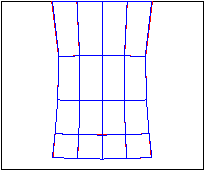
\includegraphics[width=.45\textwidth]{./graph/elasticity/stalactite-0}}
  \subfigure[{$\lambda = 10$}]{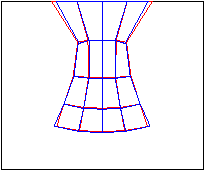
\includegraphics[width=.45\textwidth]{./graph/elasticity/stalactite-1}}
  \subfigure[{$\lambda = 100$}]{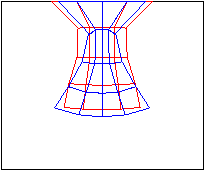
\includegraphics[width=.45\textwidth]{./graph/elasticity/stalactite-2}}
  \subfigure[{$\lambda = 1000$}]{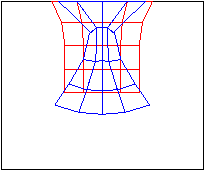
\includegraphics[width=.45\textwidth]{./graph/elasticity/stalactite-3}}
  \subfigure[{$\lambda = 10000$}]{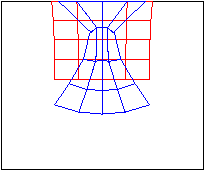
\includegraphics[width=.45\textwidth]{./graph/elasticity/stalactite-4}}
  \subfigure[{$\lambda = 100000$}]{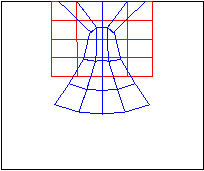
\includegraphics[width=.45\textwidth]{./graph/elasticity/stalactite-5}}
  \caption{Approximation with standard finite elements (red) and
    ``good'' elements (blue) for $\mu=1$ and different values of
    $\lambda$.}
  \label{fig:elasticity-compressibility}
\end{figure}

\begin{example}
  In a second example, we cook up a right hand side function $\vf$
  such that we know the solution to the Lamé-Navier equations. Indeed,
  we take a given solution $\vu$ and apply the differential operator
  to compute $\vf$.

  The \cref{fig:elasticity-locking} shows the $H^1$-seminorm of the
  error over the mesh size (represented by its negative dyadic
  logarithm). The black triangle denotes the convergence order $h$,
  the expected convergence of the bilinear finite elements used in
  this example.

  We see that for $\lambda=1$ and $\lambda=10$, we get the expected
  curves with the correct convergence rate. For larger values of
  $\lambda$ things seem to go wrong. There is no convergence in the
  beginning, but it seems that the expected rates are recovered on
  finer meshes.
\end{example}

\begin{figure}[tp]
  \centering
  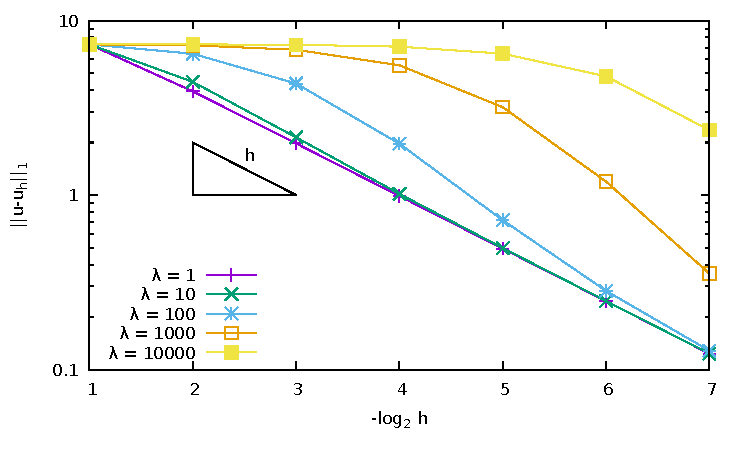
\includegraphics[width=.9\textwidth]{mixed/graph/elasticity/locking}
  \caption{Errors for a manufactured solution with different values of $\lambda$.}
  \label{fig:elasticity-locking}
\end{figure}

\begin{intro}
  As we could see in the preceding examples, approximation
  of the solution to the Lamé-Navier equations becomes difficult, if
  $\lambda \gg \mu$. In this case, the material is called almost
  incompressible, since the divergence measures compression or
  dilation and the dominating divergence term forces the divergence of
  the solution to be small. These cases are important in engineering
  and they initiated a lot of the research that resulted in the topics
  of this class. The phenomenon observed here, that the approximation
  of the solution to an elasticity problem deteriorates with
  increasing $\lambda$ is called \define{locking}.
\end{intro}

\begin{Problem}{divergence-q1}
  On $\domain = (-1,1)^2$ use the finite element mesh
  \begin{center}
  \includegraphics[width=.3\textwidth]{./fig/patch1m.tikz}, 
  \end{center}
  and on each cell the bilinear shape function space $\Q_1$, that is
  \begin{gather}
    \vV_h = \bigl\{ \vv\in \vH^1_0(\domain) \;\big|\;
    \vv_{|\cell_i} \in \Q_1\quad i=1,2,3,4\bigr\}.
  \end{gather}
  Show that for functions in $\vV_h$ there holds
  \begin{gather}
    \norm{\div \vv_h}_{L^2(\domain)} = 0
    \qquad\Rightarrow\qquad
    \vv_h = 0.
  \end{gather}
\end{Problem}
\subsection{A mixed formulation}

\begin{Definition}{robust-discretization}
  We call a discretization of a parameterized (system of) PDE robust
  with respect to the parameters or simply \define{robust}, if in an
  error estimate of the abstract form
  \begin{gather}
    \norm{u-u_h}_X \le c h^\alpha \norm{u}_Y
  \end{gather}
  the constant $c$ is independent of the parameters.
\end{Definition}

A way to approach this problem is the introduction of an auxiliary variable
\begin{gather}
  p = -\lambda \div u.
\end{gather}
Entering this definition into the Lamé-Navier equations, we obtain
the following weak formulation.

\begin{Definition}{displacement-pressure}
  The \define{displacement-pressure formulation} of the Lamé-Navier
  equations reads: find a pair $(u,p) \in V\times Q$ such that
  \begin{subequations}
  \begin{gather}
    \label{eq:lame-navier-mixed}
    \begin{aligned}
      2\mu\form(\strain u, \strain v) &- \form(p,\div v) &=&\form(f,v)
      &\forall v&\in V = \vH^1_0(\domain)\\
      -\form(q,\div u) &-\tfrac1\lambda \form(p,q) &=&0
      &\forall q&\in Q \subset L^2(\domain).\\
    \end{aligned}
  \end{gather}
  \pause
  Equivalently, we write this in a single equation as
  \begin{multline}
    2\mu\form(\strain u, \strain v) - \form(p,\div v)
    - \form(q,\div u) -\tfrac1\lambda \form(p,q)
    = \form(f,v)
    \\
    \qquad\forall v\in V, q\in Q,
  \end{multline}
  \pause
  or in the nonsymmetric, (semi-)definite version
  \begin{multline}
    2\mu\form(\strain u, \strain v) + \form(p,\div v)
    - \form(q,\div u) +\tfrac1\lambda \form(p,q)
    = \form(f,v)
    \\
    \qquad\forall v\in V, q\in Q,
  \end{multline}    
  \end{subequations}
\end{Definition}

\begin{remark}
  The three forms have different purposes and will be used
  accordingly. The first one highlights the fact that we now have a
  system of equations, each equation tested with its own test
  function. The second and third stress the fact that we now have a
  bilinear form on the product space $X=V\times Q$.
  
  The second form is symmetric, but we will see later that is
  indefinite. Thus, non of our tools from functional analysis
  apply. In contrast, the third form is nonsymmetric, but we have
  \begin{multline}
    2\mu\form(\strain u, \strain u) + \form(p,\div u)
    - \form(p,\div u) +\tfrac1\lambda \form(p,p)
    \\
    = 2\mu\form(\strain u, \strain u) + \tfrac1\lambda \form(p,p)
    \ge \tfrac{2\mu}{c_K} \norm{u}_{H^1}^2 + \tfrac1\lambda \form(p,p).
  \end{multline}
  Thus, we have ellipticity with respect to the norm
  \begin{gather}
    \norm{(u,p)}_X^2 = \norm{u}_{H^1}^2 + \norm{p}_{L^2}^2.
  \end{gather}
  Nevertheless, the ellipticity constant depends on $\lambda$, and for
  large $\lambda$, we loose sharpness of estimates again.
\end{remark}

\begin{Definition}{lame-navier-strong}
  Integrating the first equation by parts, we obtain the
  \textbf{strong form} of the \putindex{displacement-pressure
    formulation}
  \begin{gather}
    \arraycolsep.2ex
    \begin{matrix}
% Check signs
      - 2\mu \div \strain u &+& \nabla p &=& f \\
      \div u &+& \tfrac1\lambda p &=& 0
    \end{matrix}
  \end{gather}
\end{Definition}


%%%%%%%%%%%%%%%%%%%%%%%%%%%%%%%%%%%%%%%%%%%%%%%%%%%%%%%%%%%%%%%%%%%%%%
%%%%%%%%%%%%%%%%%%%%%%%%%%%%%%%%%%%%%%%%%%%%%%%%%%%%%%%%%%%%%%%%%%%%%%
\section{Stokes equations}

\begin{intro}
  When we write the Lamé-Navier equations in \putindex{displacement-pressure formulation} according to
  \slideref{Definition}{displacement-pressure}, there is no
  parameter $\lambda$ tending to infinity when the material becomes
  less and less compressible. Instead, there is the parameter
  $1/\lambda$ tending to zero. Thus, we can simply consider the case
  of incompressible material by setting $1/\lambda=0$ or, in our
  abstract framework~\eqref{eq:mixedintro:1} setting $c(\cdot,\cdot) = 0$. The
  resulting system is not only important for incompressible
  elasticity, but also models the slow flow of a very viscous liquid,
  so called \putindex{creeping flow}.
\end{intro}

\begin{Definition}{stokes-eq1}
  The \define{Stokes equations} in strong form are
    \begin{gather}
      \label{eq:mixedintro:stokes-strong1}
      \arraycolsep.2ex
      \begin{matrix}
        -2\mu \div \strain \vu &+& \nabla p &=& \vf \\
        \div \vu && &=& 0.
      \end{matrix}
    \end{gather}
    In weak form, they are: find $\vu\in \vV \subset \vH^1(\domain)$
    and $p\in Q \subset L^2(\domain)$ such that
  \begin{gather}
    \label{eq:mixedintro:stokes-weak1}
    \begin{aligned}
      2\mu\form(\strain \vu, \strain \vv) &- \form(\div \vv,p) &=&\form(\vf,\vv)
      + \text{bdry}
      &\forall \vv&\in \vV\\
      -\form(\div \vu,q) & &=&0+ \text{bdry}
      &\forall q&\in Q.\\      
    \end{aligned}
  \end{gather}
  The subspaces $\vV$ and $Q$ are determined by boundary conditions.
\end{Definition}

\begin{Definition}{solenoidal}
  A vector-valued function $\vu$ is called \define{divergence-free} or
  \define{solenoidal}, if there holds
  \begin{gather}
    \div \vu = 0.
  \end{gather}
  Flow described by a solenoidal function is called
  \define{incompressible}.
\end{Definition}

\begin{Lemma}{stokes-equivalence}
  Let $\vV=\vH^1_0(\domain)\cap \vH^2(\domain)$. Then, for any
  solenoidal function $\vu\in vV$ there holds
  \begin{gather}
    \label{eq:mixedintro:6}
    2\mu\form(\strain \vu, \strain \vv) = \mu\form(\nabla \vu, \nabla \vv)
    \qquad\forall \vv\in \vV.
  \end{gather}
\end{Lemma}

\begin{proof}
  We have ('$:$' denoting the \putindex{double contraction} of
  \putindex{Frobenius inner product})
  \begin{align}
    \strain \vu: \strain \vv
    &= \frac14\sum_{i,j=1}^d\left[ (\d_i u_j+\d_j u_i) (\d_i v_j+\d_j v_i)
      \right]
    \\
    &= \frac12\sum_{i,j=1}^d\left[ \d_i u_j\d_iv_j + \d_i u_j\d_j v_i\right].
  \end{align}
  The first term is the desired result, thus we have to eliminate the
  other one. We integrate by parts to obtain
  \begin{align}
    \int_\domain \d_i u_j\d_j v_i \dx
    &= - \int_\domain \d_{ij}u_j v_i \dx
%     \\ &
    = \int_\domain \d_j u_j \d_i v_i \dx 
  \end{align}
  Entering in the
  previous equation and summing over $i$ and $j$, we obtain
  \begin{gather}
    2(\strain \vu,\strain \vv)
    = (\nabla \vu,\nabla \vv)+(\div \vu,\div \vv)
                           = (\nabla \vu,\nabla \vv).
  \end{gather}
\end{proof}

\begin{intro}
  In order to simplify subsequent discussion, it is customary to use
  the previous lemma to simplify the Stokes equations and to replace
  the strain tensor by the gradient. As a result, we can avoid the use
  of a Korn inequality and operate directly with the inner product of
  $\vH^1$. We note though that this formulation, while mathematically
  simpler, is physically wrong if $\vu\neq \vH^1_0(\domain)$, that is,
  having nonzero boundary values.
\end{intro}

\begin{Definition}{stokes-eq2}
  The simplified \define{Stokes equations} in strong form are
    \begin{gather}
      \label{eq:mixedintro:stokes-strong2}
      \arraycolsep.2ex
      \begin{matrix}
        - \nu \Delta \vu &+& \nabla p &=& \vf \\
        \div \vu && &=& 0.
      \end{matrix}
    \end{gather}
    In weak form, they are: find $\vu\in V \subset \vH^1(\domain)$
    and $p\in Q \subset L^2(\domain)$ such that
  \begin{gather}
    \label{eq:mixedintro:stokes-weak2}
    \begin{aligned}
      \nu\form(\nabla \vu, \nabla \vv) &- \form(\div \vv,p) &=&\form(\vf,\vv)
      + \text{bdry}
      &\forall \vv&\in \vV\\
      -\form(\div \vu,q) & &=&0+ \text{bdry}
      &\forall q&\in Q.\\      
    \end{aligned}
  \end{gather}
  The subspaces $V$ and $Q$ are determined by boundary conditions.
\end{Definition}

\begin{Definition}{stokes-boundary2}
  Typical boundary conditions for the Stokes problem are
  \begin{xalignat}3
    \text{no-slip:}&& \vu &= 0,\\
    \text{free:}&& \d_n \vu + p \n &= 0 ,\\
    \text{slip:}&& \vu_n &= 0 & \d_n \vu_\tau &= 0,\\
    \text{friction:}&& \vu_n &= 0 & \d_n \vu_\tau &= \alpha \vu_\tau.
  \end{xalignat}
  Here, $\vu_n$ and $\vu_\tau$ are the normal and tangential components of
  $\vu$ at the boundary.
\end{Definition}

\begin{remark}
  Very much the same way as for elliptic equations, boundary
  conditions on the function $\vu$ itself are essential boundary
  conditions which have to be incorporated into the space $V$, while
  those involving normal derivatives are the result of integration by
  parts and thus of the type of natural boundary conditions.

  All of the conditions above can also be imposed with nonzero data,
  where the physical meaning of such a condition might be debatable in
  some cases. Mathematically, inhomogeneous essential boundary
  conditions are achieved by lifting an arbitrary function with this
  boundary condition and modifying the right hand side of the
  equation, while inhomogeneous conditions on the normal derivative
  are implemented by boundary integrals on the right hand side.
\end{remark}

\begin{remark}
  Physically, the condition $\vu_n=0$ models an impermeable wall. It
  says in particular, that no mass is lost through this boundary and
  is thus related to the first principle of mass conservation.

  The conditions on the tangential velocity model the fact that
  molecules very close to the wall stick to the wall. While this claim
  is not supported by a first principle, it has been verified by
  measurements to very high accuracy. Nevertheless, in the study of
  turbulent flow, a friction condition comes up quite naturally.
\end{remark}

\begin{Lemma}{divergence-compatibility}
  For any solenoidal $\vu$ function there holds
  \begin{gather}
    \int_{\d\domain} \vu\cdot \n\ds = 0.
  \end{gather}
  Furthermore, if the space $\vV$ in the Stokes equations is chosen such that for any $\vv\in \vV$ there holds $\vv_n=0$ on the whole
  boundary $\d\domain$, then the pressure $p$ is determined by the
  Stokes equations only up to a constant.
\end{Lemma}

\begin{proof}
  The first statement is simple application of the Gauss theorem
  \begin{gather}
    \int_{\domain} \div \vu\dx = \int_{\d\domain} \vu\cdot \n\ds.
  \end{gather}
  For the second statement, we note that the only term in the
  equations which determines the pressure is $\form(\div \vv,
  p)$. Integrating by parts and using the boundary condition, we
  obtain
  \begin{gather}
    \int_\domain \div \vv\,p\dx
    = -\int_\domain \vv\cdot\nabla p\dx +
    \int_{\d\domain} \vv\cdot \n \,p\ds
    = -\int_\domain \vv\cdot \nabla p\dx.
  \end{gather}
  Since the gradient of a constant is zero, we can add any constant
  function to a given solution $p$ without changing the term
  $\form(\div \vv,p)$, thus leaving $p$ determined only up to a
  constant.
\end{proof}

\begin{Notation}{pressure-constant}
  If in Definition~\ref{Definition:stokes-eq2} the space $\vV$ is chosen
  such that for all $\vv\in \vV$ there holds $\vv\cdot \n =0$ on the whole
  boundary $\d\domain$, then the pressure solution $p$ cannot be
  determined uniquely in $L^2(\domain)$. In such cases, we choose the
  pressure space
  \begin{gather}
    L^2_0(\domain) = L^2(\domain)/\R
    = \biggl\{q\in L^2(\domain)\bigg| \int_\domain q\dx = 0\bigg\}. 
  \end{gather}
\end{Notation}

\begin{remark}
  As we could see from the preceding lemma, solvability of
  equation~\eqref{eq:mixedintro:stokes-weak2} depends on some
  compatibility of the spaces $\vV$ and $Q$ we had not seen in the
  elliptic case. Indeed, we need a whole new tool from functional
  analysis to replace the Lax-Milgram lemma. This tool will be studied
  in Chapter~\ref{sec:mixed-wellposedness}.
\end{remark}


%%% Local Variables: 
%%% mode: latex
%%% TeX-master: "main"
%%% End: 
